% =====================================================================
%  CAPÍTULO 2. DISEÑO E IMPLEMENTACIÓN DEL MODELO (SGC)
%  Estructura del modelo científico según el Taller 4:
%  conceptualización y alcance -> factores y variables -> procedimiento
%  y toma de observaciones -> validación -> contraste de hipótesis.
% =====================================================================
\chapter{DISEÑO E IMPLEMENTACIÓN DEL SISTEMA DE GESTIÓN DE LA CALIDAD}
\label{cap:diseno}

% ---------------------------------------------------------------------
\section{Conceptualización y alcance del modelo de investigación}

El modelo de investigación compara el desempeño del proceso constructivo de la losa alivianada en dos condiciones:
\begin{itemize}
  \item sin un sistema de gestión de la calidad (primera losa, ya ejecutada), y
  \item con el SGC propuesto (segunda losa).
\end{itemize}
El efecto se mide mediante el costo unitario, el desperdicio de materiales y el costo de no calidad (Figura~\ref{fig:modelo} y Tabla~\ref{tab:fases}).

\begin{figure}[H]
\centering
\caption{Esquema del modelo de investigación}
\label{fig:modelo}
\begin{tikzpicture}[
  caja/.style={draw, rounded corners=2pt, align=center, text width=3.4cm,
               minimum height=2.1cm, font=\small, fill=gray!8},
  flecha/.style={-{Stealth[length=3mm]}, thick}]
  \node[caja] (o1) {\textbf{$O_1$: línea base}\\ Primera losa\\ sin SGC\\ 41 paños\\ 1.109,84~\mdos{}};
  \node[caja, right=0.4cm of o1] (x) {\textbf{$X$: aplicación}\\ \textbf{del SGC}\\ Plan de la calidad,\\ PPI y control\\ de materiales};
  \node[caja, right=0.4cm of x] (o2) {\textbf{$O_2$: posprueba}\\ Segunda losa\\ con SGC\\ (o simulación\\ \emph{ex ante})};
  \node[caja, right=0.4cm of o2] (h) {\textbf{Contraste}\\ Prueba \emph{t}\\ o Wilcoxon\\ $\alpha = 0{,}05$};
  \draw[flecha] (o1) -- (x);
  \draw[flecha] (x) -- (o2);
  \draw[flecha] (o2) -- (h);
\end{tikzpicture}
\nota{Elaboración propia.}
\end{figure}

\begin{table}[H]
\caption{Fases del modelo de investigación}
\label{tab:fases}
\begin{tabularx}{\linewidth}{@{}P{3.0cm}LP{4.0cm}P{1.7cm}@{}}
\toprule
\textbf{Fase} & \textbf{Actividades} & \textbf{Productos} & \textbf{Objetivo} \\
\midrule
1. Diagnóstico & Análisis documental, diagnóstico de brechas ISO~9001 y entrevistas & No conformidades y causas & OE1 \\
2. Línea base ($O_1$) & Cuantificación de consumos, desperdicios y costos de la primera losa & Índices de desperdicio y costo de no calidad & OE2 \\
3. Diseño ($X$) & Plan de la calidad, PPI, procedimientos y formatos & SGC del ítem & OE3 \\
4. Aplicación ($O_2$) & Implementación en la segunda losa o simulación & Índices con el SGC & OE4 \\
5. Contraste y validación & Pruebas estadísticas y juicio de expertos & Aceptación o rechazo de la hipótesis & OE5 \\
\bottomrule
\end{tabularx}
\nota{Elaboración propia.}
\end{table}

% ---------------------------------------------------------------------
\section{Caracterización del caso de estudio}

\subsection{Ubicación y descripción del edificio}
El Edificio de Posgrado se emplaza en la Ciudadela Universitaria de la UATF, en el sector noreste, junto al edificio del Vicerrectorado, sobre la avenida Las Banderas de la ciudad de Potosí, a 3650~m~s.~n.~m. El proyecto tiene seis niveles. Por el desnivel del terreno, la planta baja presenta desniveles en tres sectores. La fase en estudio comprende la obra gruesa (fundaciones, columnas, vigas, losas alivianadas y escaleras de hormigón armado) hasta la tercera losa. También incluye la colocación de ductos y cajas eléctricas y sanitarias embebidas en losas y vigas \parencite{uatf_item13}.

\subsection{Datos contractuales y cronología}

\begin{table}[H]
\caption{Cronología de la ejecución del proyecto}
\label{tab:cronologia}
\begin{tabularx}{\linewidth}{@{}P{3.2cm}L@{}}
\toprule
\textbf{Fecha} & \textbf{Hecho} \\
\midrule
06/05/2025 & Inicio de obra; plazo de 270 días calendario y monto de Bs~3.367.031,95. \\
12/06/2025 & FANCESA comunica la paralización temporal de su producción por falta de diésel. \\
04/09/2025 -- 08/12/2025 & Periodo de la Planilla de avance N.\textsuperscript{o}~2 (95 días trabajados). \\
09/10/2025 & Pronunciamiento de la Cámara de la Construcción de Tarija sobre el alza del cemento. \\
27/11/2025 & Certificados de calidad de viguetas pretensadas (PRETENSA) y de plastoformo (UNICON). \\
05/12/2025 & Certificado de laboratorio N.\textsuperscript{o}~000293 (probetas de columnas y vigas). \\
08/12/2025 & Avance acumulado del 56,97~\%; contrato modificado a Bs~3.610.125,43 y plazo de 360 días. \\
05/01 y 10/02 \pendiente{año} & Paralización por solicitud de resolución concertada del contrato y respuesta favorable de la UATF. \\
Planilla N.\textsuperscript{o}~3 & Resolución del contrato: avance del 57,48~\% y 1.109,84~\mdos{} de losa ejecutados. \\
\bottomrule
\end{tabularx}
\nota{Elaborado con base en \textcite{uatf2025pao2}, \textcite{uatf_pao3}, \textcite{uatf_item13}, \textcite{fancesa2025} y \textcite{cadeco2025}.}
\end{table}

\subsection{Sistema de losa: planos, especificaciones y certificados}
La primera losa se divide en 41 paños, de 1,40 a 52,38~\mdos{} cada uno, que suman 1.109,84~\mdos{} (Figura~\ref{fig:geometria}). Las características del sistema según los documentos del proyecto se resumen en la Tabla~\ref{tab:sistema}.

\begin{figure}[H]
\centering
\caption{Geometría y paños de la primera losa del Edificio de Posgrado}
\label{fig:geometria}
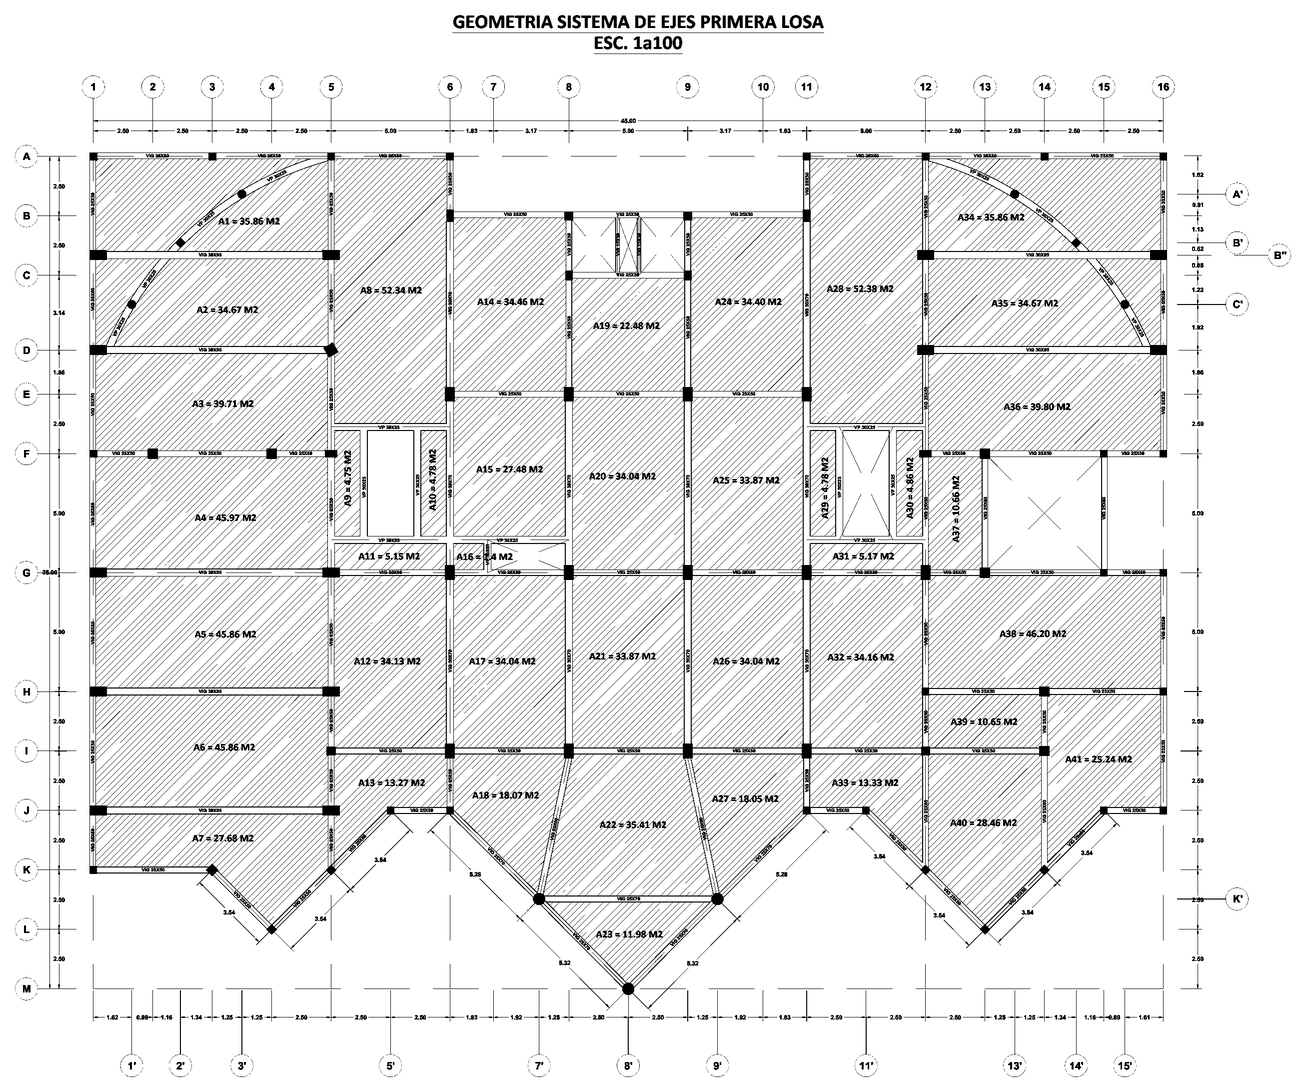
\includegraphics[width=\linewidth]{plano01_geometria_primera_losa}
\nota{Tomado del Plano~01 «Geometría sistema de ejes primera losa» (escala original 1:100). Las áreas A1 a A41 corresponden a los paños de losa computados.}
\end{figure}

\begin{table}[H]
\caption{Características de la losa alivianada según los documentos del proyecto}
\label{tab:sistema}
\begin{tabularx}{\linewidth}{@{}P{4.2cm}LP{3.6cm}@{}}
\toprule
\textbf{Característica} & \textbf{Valor} & \textbf{Fuente} \\
\midrule
Espesor total & 25~cm (20~cm + 5~cm de carpeta) & ET; certificado PRETENSA \\
Separación entre ejes de viguetas & 50~cm & Certificado PRETENSA \\
Luz máxima de vigueta & 7,50~m (simplemente apoyada) & Certificado PRETENSA \\
Sobrecarga admisible & 400~kg/\mdos{} & Certificado PRETENSA \\
Hormigón de viguetas & 350 a 400~kg/cm\textsuperscript{2} & ET \\
Hormigón de carpeta y nervios & H25, f'c~=~250~kg/cm\textsuperscript{2}, cemento $\geq$~400~kg/\mtres{} & ET \\
Armadura de distribución & $\phi$6~c/20~cm en ambas direcciones & Plano~02 \\
Complemento (según ET) & Plastoformo de 100~$\times$~50~$\times$~20~cm & ET \\
Complemento (suministrado) & Plastobloq de 20~$\times$~100~$\times$~44~cm, densidad 10~kg/\mtres{} & Certificado UNICON \\
\bottomrule
\end{tabularx}
\nota{ET: especificaciones técnicas del proyecto \parencite{uatf_et}. Certificados: \textcite{pretensa2025} y \textcite{unicon2025}.}
\end{table}

% ---------------------------------------------------------------------
\section{Definición de factores y variables}
\label{sec:variables}

Las variables, sus dimensiones e indicadores se detallan en el Anexo~\ref{anx:operacionalizacion}. Los indicadores principales se calculan de la siguiente manera.

\textbf{Índice de desperdicio del material $i$:}
\begin{equation}
  IDM_i = \frac{Q_{\text{real},i} - Q_{\text{teórica},i}}{Q_{\text{teórica},i}} \times 100
  \label{eq:idm}
\end{equation}
donde $Q_{\text{real},i}$ es la cantidad consumida (entregada menos sobrante recuperable) y $Q_{\text{teórica},i}$ es la cantidad según planos y cómputos.

\textbf{Costo unitario a precios constantes del contrato:}
\begin{equation}
  CU = \frac{\sum_{j} Q_{j}\, p_{j} + C_{MO} + C_{EQ}}{A}
  \label{eq:cu}
\end{equation}
donde $Q_j$ es la cantidad real del insumo $j$, $p_j$ su precio en el análisis de precios unitarios del contrato, $C_{MO}$ y $C_{EQ}$ los costos de mano de obra y equipo, y $A$ la superficie ejecutada (\mdos{}).

\textbf{Costo de la calidad y costo de no calidad (modelo PAF):}
\begin{equation}
  CC = C_{P} + C_{E}, \qquad CNC = C_{FI} + C_{FE}, \qquad \%CNC = \frac{CNC}{C_{\text{ítem}}} \times 100
  \label{eq:cnc}
\end{equation}
donde $C_P$ son los costos de prevención, $C_E$ los de evaluación, $C_{FI}$ los de fallas internas (desperdicio, retrabajo y reparaciones) y $C_{FE}$ los de fallas externas (sobremediciones corregidas, ampliaciones y multas).

\textbf{Reducción relativa del costo en el paño homólogo $k$:}
\begin{equation}
  r_k = \frac{CU_{\text{sin},k} - CU_{\text{con},k}}{CU_{\text{sin},k}}
  \label{eq:reduccion}
\end{equation}

\guia{Si un material solo puede medirse por vaciado o por losa completa (por ejemplo, el hormigón), la unidad de análisis de ese indicador será el vaciado y no el paño.}

% ---------------------------------------------------------------------
\section{Población y muestra}
La población está formada por las losas alivianadas del edificio (3.344,44~\mdos{}). La unidad de análisis es el paño de losa. Se adopta una muestra no probabilística censal: los 41 paños de la primera losa (preprueba) y los paños homólogos de la segunda losa (posprueba). Así se compara cada paño con otro de la misma geometría.

\guia{Confirmar con los planos de la segunda losa que los paños son homólogos (misma geometría y cantidad de viguetas). Si no lo son, comparar con muestras independientes (prueba \emph{t} para muestras independientes o U de Mann-Whitney).}

% ---------------------------------------------------------------------
\section{Diagnóstico de la situación actual (línea base)}

\subsection{Diagnóstico de brechas frente a la norma ISO~9001:2026}
\guia{Aplicar la lista de verificación (Anexo~\ref{anx:instrumentos}) a la contratista y a la Supervisión. Calificar cada requisito aplicable de las cláusulas 4 a 10 (cumple, cumple parcialmente o no cumple) y calcular el porcentaje de cumplimiento por cláusula. Presentar los resultados en una tabla y un gráfico de barras.}

\subsection{Análisis documental de la primera losa}
\label{sec:analisis-documental}

La revisión preliminar de los documentos de la obra muestra los siguientes hallazgos.

\textbf{a) Control de la resistencia del hormigón.} El certificado de laboratorio N.\textsuperscript{o}~000293 (Tabla~\ref{tab:probetas}) es el único registro de ensayos de compresión adjunto a la Planilla N.\textsuperscript{o}~2. Comprende doce probetas de 15~$\times$~30~cm (6~$\times$~12~pulg) de columnas y vigas, ensayadas entre los 55 y 76 días y «proyectadas» a 28 días con un factor de tiempo \parencite{labuatf2025}. Todos los valores superan f'c~=~250~kg/cm\textsuperscript{2}. Sin embargo:
\begin{enumerate*}[label=(\roman*)]
  \item no hay probetas de la losa alivianada;
  \item los ensayos no se hicieron a la edad especificada de 28 días;
  \item las probetas fueron elaboradas por la propia contratista, sin muestreo independiente; y
  \item cuatro de los doce valores proyectados están por debajo de 260~kg/cm\textsuperscript{2}, con poco margen sobre la resistencia especificada.
\end{enumerate*}

\begin{table}[H]
\caption{Resultados del certificado de laboratorio N.\textsuperscript{o}~000293}
\label{tab:probetas}
\begin{tabularx}{\linewidth}{@{}LQ{1.6cm}Q{1.9cm}Q{3.0cm}Q{1.3cm}Q{1.0cm}Q{1.0cm}@{}}
\toprule
\textbf{Elemento} & \textbf{N.\textsuperscript{o} probetas} & \textbf{Edad (días)} & \textbf{Resistencia proyectada a 28 días (kg/cm\textsuperscript{2})} & \textbf{Media} & \textbf{$s$} & \textbf{CV} \\
\midrule
Columnas & 10 & 55--76 & 253,6 -- 287,8 & 267,2 & 9,9 & 3,7~\% \\
Vigas & 2 & 76 & 252,0 -- 261,4 & 256,7 & 6,6 & 2,6~\% \\
Losa alivianada & 0 & --- & sin ensayos & --- & --- & --- \\
\bottomrule
\end{tabularx}
\nota{Elaborado con base en el certificado del Laboratorio de Resistencia de Materiales y Tecnología del Hormigón de la Carrera de Ingeniería Civil de la UATF \parencite{labuatf2025}. $s$: desviación estándar; CV: coeficiente de variación.}
\end{table}

\textbf{b) Requerimientos de la Supervisión.} En su informe de la Planilla N.\textsuperscript{o}~2, la Supervisión recomendó a la contratista \parencite{uatf2025pao2}:
\begin{itemize}
  \item presentar las garantías de todos los materiales empleados;
  \item realizar la rotura de probetas de los elementos vaciados;
  \item presentar las dosificaciones de los hormigones.
\end{itemize}
Es decir, al cierre del periodo no se contaba con estos controles básicos.

\textbf{c) Coherencia de los documentos técnicos.} Tres documentos describen el complemento de manera distinta:
\begin{itemize}
  \item las especificaciones técnicas exigen bloques de 100~$\times$~50~$\times$~20~cm;
  \item el corte transversal del Plano~02 acota una altura de 0,15~m;
  \item el certificado del proveedor corresponde a bloques de 20~$\times$~100~$\times$~44~cm \parencite{uatf_et,unicon2025}.
\end{itemize}
La falta de control de la información documentada y de los cambios, que exige la norma ISO~9001, es una no conformidad del sistema actual.

\textbf{d) Cantidades de materiales.} Se entregaron 2.350 piezas de plastoformo \parencite{unicon2025}. Con una separación de 50~cm entre ejes y bloques de 1,00~m de largo, el consumo teórico bruto es de 2 piezas por \mdos{}, es decir, $\approx$~2.220 piezas para 1.109,84~\mdos{} sin descontar nervios ni bordes. La diferencia preliminar es de $\approx$~130 piezas ($\approx$~6~\%).

Además, el cómputo de acero de la planilla de resolución incluye «losa alivianada: 3 $\times$ 4.171,18 kg = 12.513,54 kg», aunque solo se ejecutó una losa \parencite{uatf_pao3}.

\pendiente{verificar con la Supervisión si las 2.350 piezas corresponden solo a la primera losa, el número real de piezas colocadas y sobrantes, y a qué corresponde el factor 3 del acero.}

\subsection{No conformidades y análisis de causas}
\guia{Registrar las no conformidades encontradas en el Libro de Órdenes (fotocopias en la Planilla N.\textsuperscript{o}~2), en los informes de Supervisión y en las entrevistas. Clasificarlas por categoría: materiales, mano de obra, método, documentación, equipo y medición. Elaborar un diagrama de Pareto (frecuencia y costo) y un diagrama de Ishikawa de las causas del desperdicio y de los sobrecostos.}

\subsection{Cuantificación del desperdicio de materiales y del costo de no calidad}
\guia{Aplicar las ecuaciones \eqref{eq:idm} a \eqref{eq:cnc} a la primera losa:
\begin{enumerate}
  \item Cantidades teóricas: planos 01 a 03 y cómputos.
  \item Cantidades entregadas: notas de entrega, facturas y kardex.
  \item Cantidades pagadas: planillas de avance.
\end{enumerate}
Presentar una tabla por material (hormigón, acero, viguetas y plastoformo) con el índice de desperdicio y su costo a precios del contrato. Este es el valor de referencia ($O_1$) de la hipótesis.}
